

\subsection{Решение задачи структурного синтеза}
Для создания соответствующего робота, который может эффективно решать конкретные задачи, необходимо провести структурный синтез. То есть, мы оптимизируем характеристики робота, такие как количество ног, угол между ногами и.т.д., используя алгоритмы оптимизации.

\subsubsection{Математическая модель робота}
Геометрическая модель робота представлена в виде трехмерного параллелепипеда с несколькими ногами с каждой стороны. Каждая нога имеет постоянное смещение угла поворота относительно своей соседней ноги.

Эти параметры влияют на длину робота:
количество лап  $\gamma$; угол между соседними лапами  $x$;

\begin{eqnarray}
    \label{eq:first}
    L_{body} = 2 \cdot \text{offset}_{first\_hole} + ((\gamma - 1) \cdot\ \text{legs}_{height} \cdot sin(x) + q)
\end{eqnarray}
где $q$ сдвиг между соседними лапами.

Мы решаем мультикритериальную задачу оптимизации, где мы пытаемся максимизировать дистанцию, пройденную за фиксированное время, и минимизировать длину робота.

\begin{eqnarray}
    \label{eq:second}
    F = \beta \left( {\omega}_{1} \cdot \delta + {\omega}_{2} \cdot \frac{1}{(\gamma - 1) sin(x)}\right) +\\ \nonumber + (1 - \beta) {\delta}^{{\omega}_{1}} {\left( \frac{1}{(\gamma - 1) sin(x)}\right)}^{{\omega}_{2}}
\end{eqnarray}
где $\delta$ дистанция, $\beta$ адаптивный параметр, ${\omega}_{1,2}$ весовые коэффициенты.

Следующие параметры оптимизируются: $\gamma$, $\omega$, $q$. Последний параметр зависит не на прямую на проходимость.

\subsubsection{Разработка генетического алгоритма}
Генетический алгоритм --- это эвристический алгоритм поиска, используемый для решения задач оптимизации и моделирования путём случайного подбора, комбинирования и вариации искомых параметров с использованием механизмов, аналогичных естественному отбору в природе. Позволяет найти глобальный максимум.

Для решения задачи использовалась библиотека Deap.

\begin{algorithm}[H]
\caption{Решение задачи оптимизации\label{high_level}}
% \begin{small}
\KwIn{$\alpha$ -- количество генераций, $\beta$ -- количество индивидуумов, $\gamma$ -- количество территорий}
\KwOut{Оптимальные параметры}
\Begin{
Генерируем семейство территорий\;
Инициализируем первую популяцию роботов случайными параметрами\;
\For{$i = 0$ \KwTo $\alpha$}{
\For{$j = 0$ \KwTo $\beta$}{
$distance = 0$\;
\For{$k = 0$ \KwTo $\gamma$}{
start simulation\;
$distance += cur\_distance$\;
}
$avg\_distance = distance / \gamma$\;
Вычисляем фитнесс функцию\;
}
Выбираем лучших родителей\;
Производим кроссовер у лучших родителей\;
Делаем мутацию\;
}
}
% \end{small}
\end{algorithm}

\subsubsection{Результаты}
Было два этапа результатов. На первом этапе мы стремились найти только одного лучшего робота, только для местности T1. На втором этапе мы хотели видеть зависимость от разных типов ландшафтов при меньшем количестве индивидуальностей.

Первый этап: каждый робот проходил 10 разных ландшафтов по 9 секунд каждую.
В результате нашей работы мы получили следующие результаты: после 11 поколений и 200 индивидуумов в начальной популяции лучший робот имеет 6 ног с каждой стороны (всего 12 ножек), угол 73 градусов между ногами и смещение волны 163 градусов между сторонами. С такими характеристиками роботу удалось пройти 5,21 метра, тогда как начальное население могло пройти меньше 2.

Вторая фаза: она имеет те же параметры, что и первая фаза, исключая количество людей. На этом этапе насчитывается 55 индивидуумов.
Полученные результаты показаны в таблице \cref{tabular:Table2}.
\begin{figure}[ht!]
    \begin{subfigure}{0.33\textwidth}
    \centering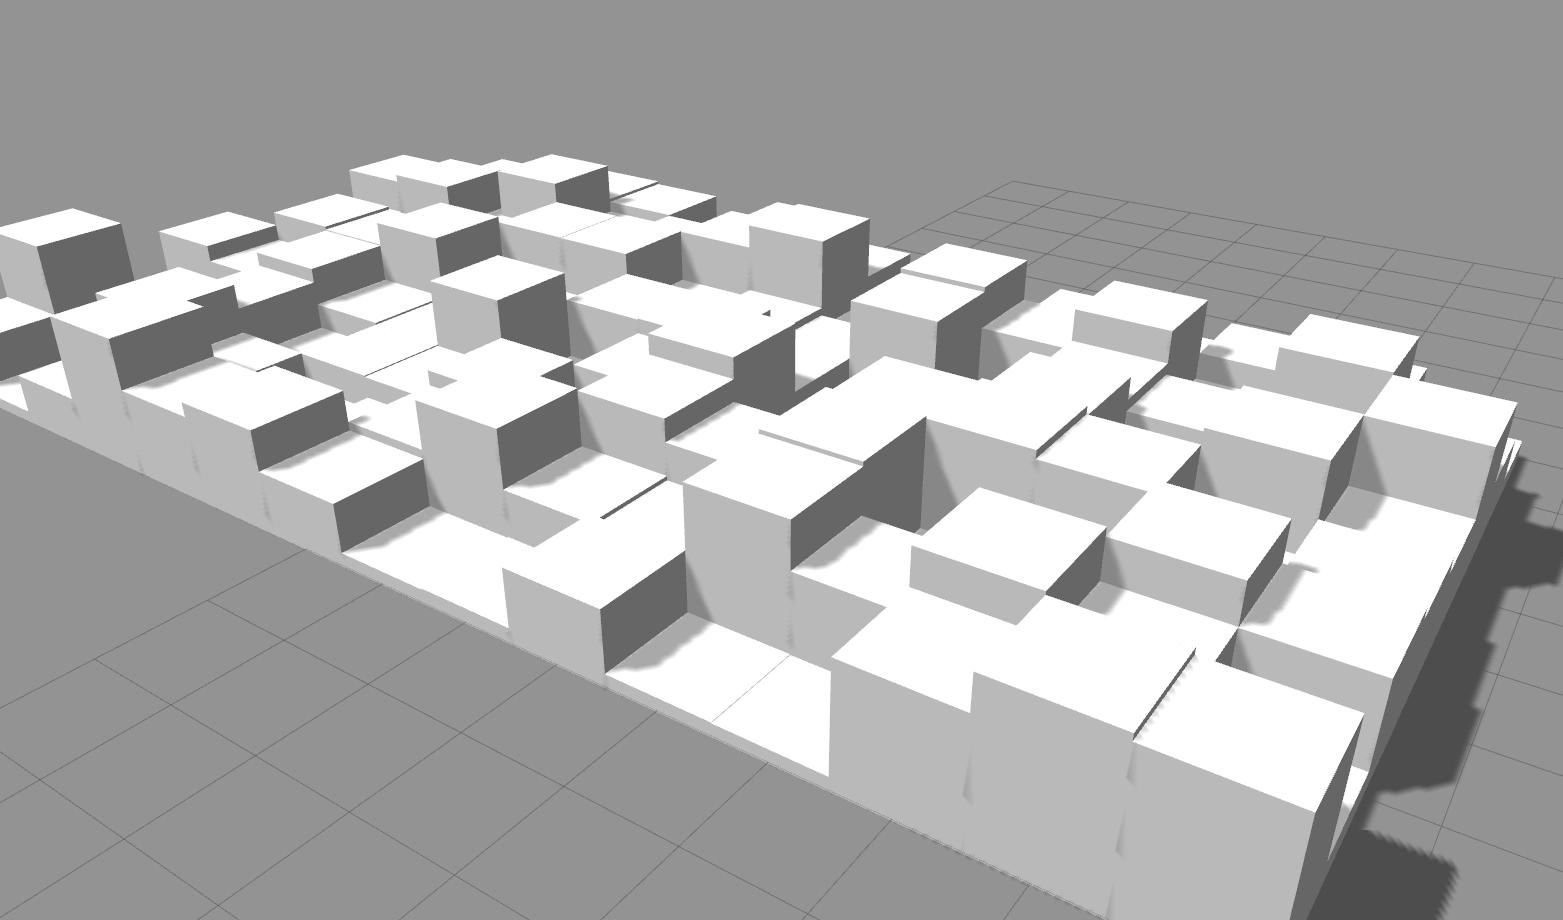
\includegraphics[width=0.8\textwidth]{terrain_1} 
    \caption{T1: 3D-боксы с равномерным распределением высоты}
    \label{fig:terrain_1}
    \end{subfigure}
    \begin{subfigure}{0.33\textwidth}
    \centering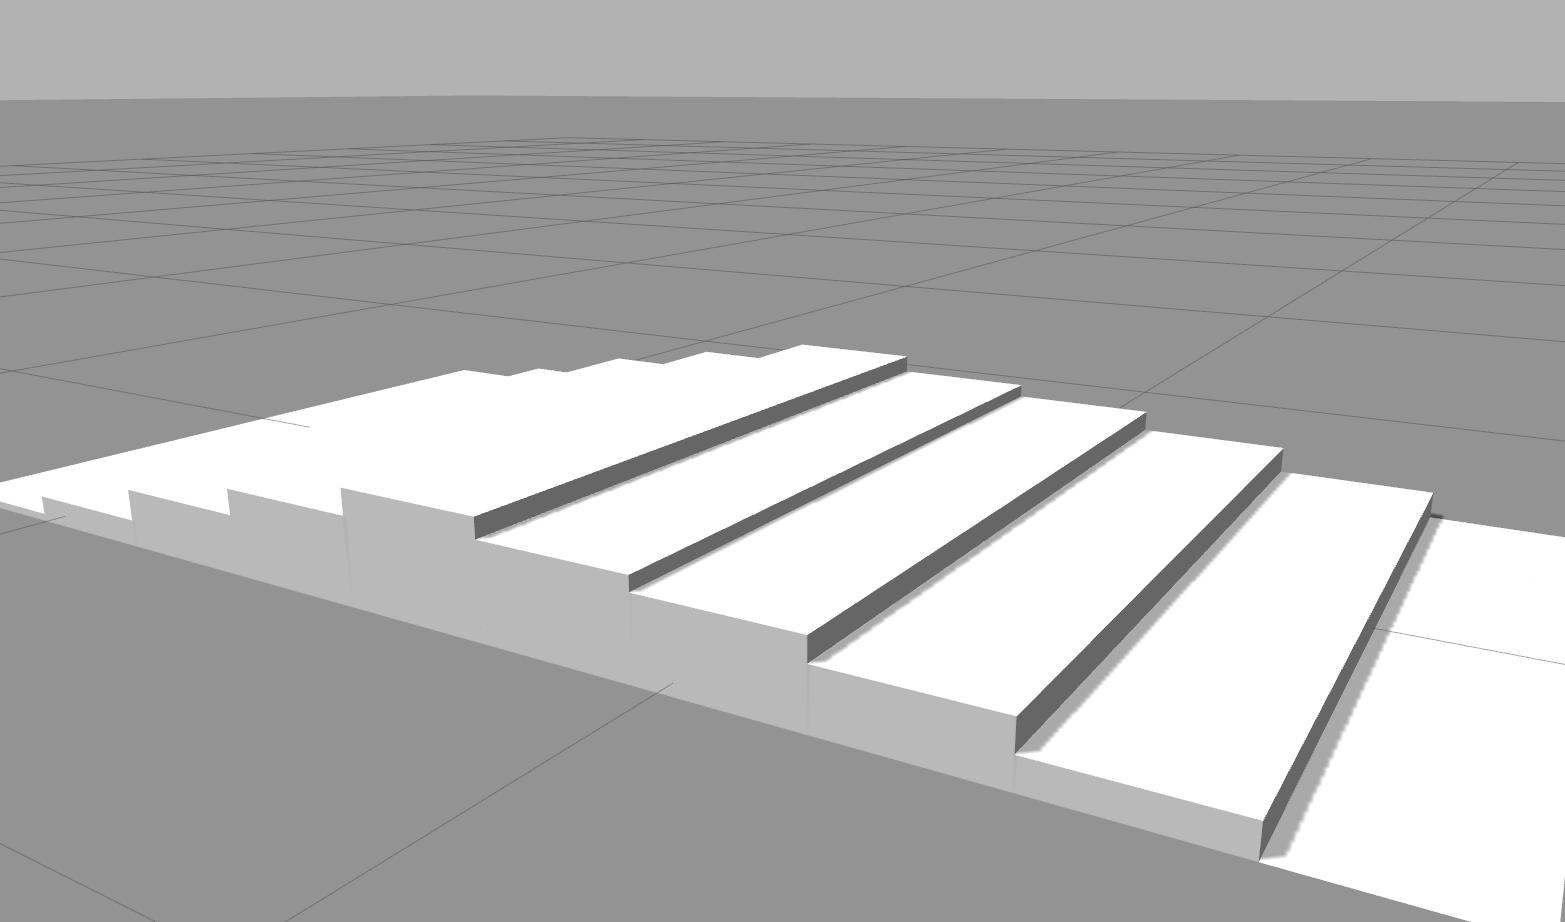
\includegraphics[width=0.8\textwidth]{terrain_2} 
    \caption{T2: 2D-полосы с гауссовой функциональной высотой}
    \label{fig:terrain_2}
    \end{subfigure}
    \begin{subfigure}{0.33\textwidth}
    \centering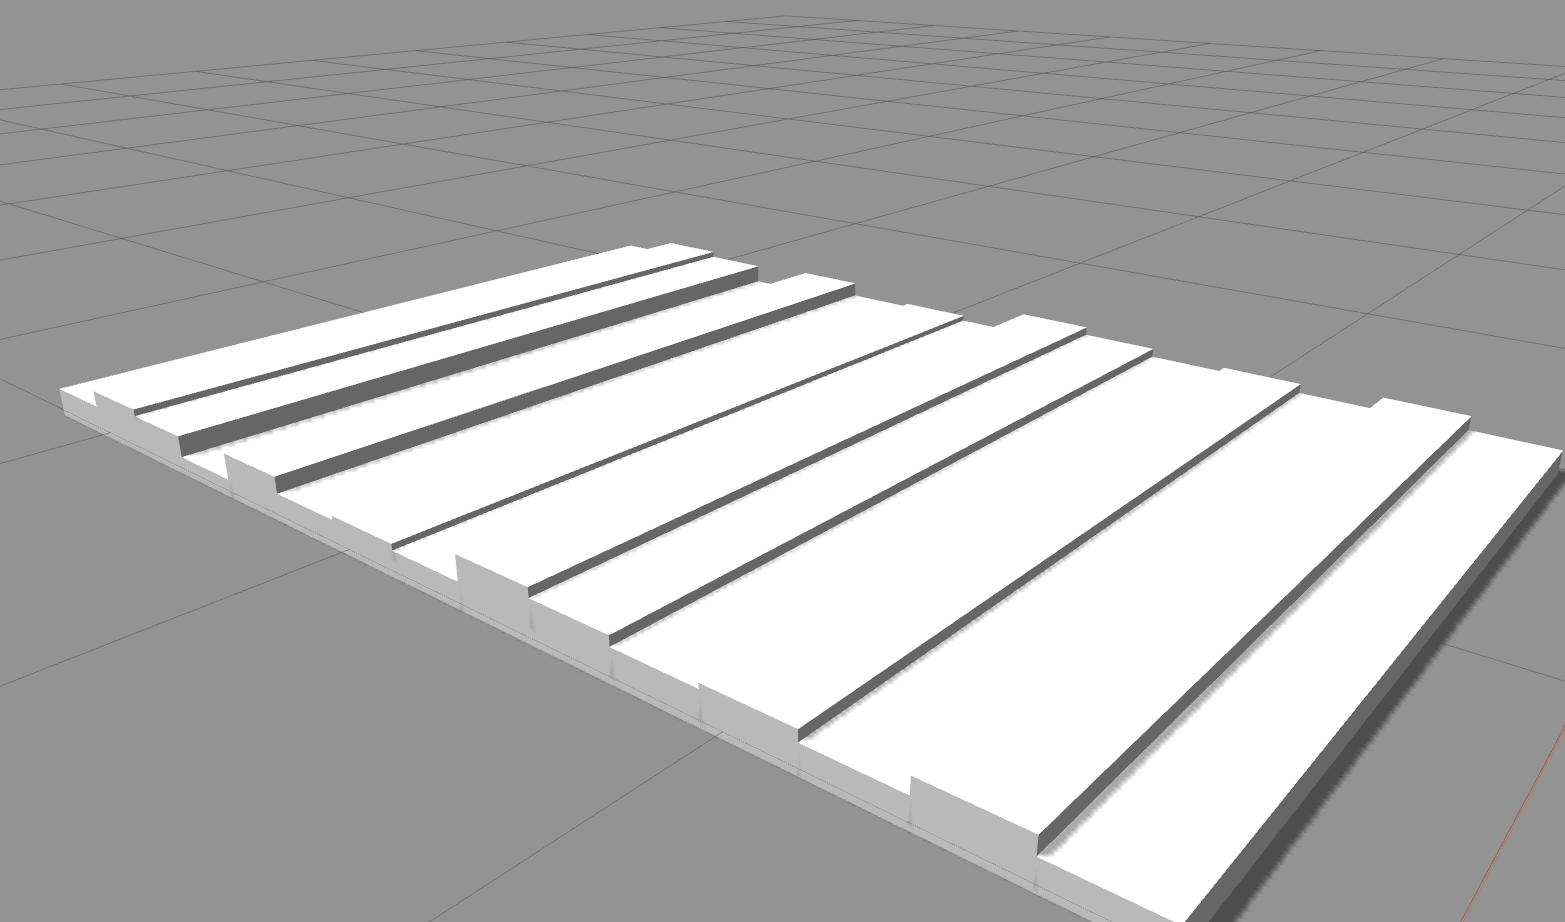
\includegraphics[width=0.8\textwidth]{terrain_3}
    \caption{T3: 2D-полосы с распределением высоты по гауссовской функции)}
    \label{fig:terrain_3}
    \end{subfigure}
     
    \caption{Примеры сгенерированных территорий}
    \label{fig:terrains}
\end{figure}
\vspace{-0.5cm}

\begin{table}[ht!]
\caption{Зависимость между статистикой значения пригодности (средняя, std) и типами ландшафта}
\label{tabular:Table2}
\begin{center}
\begin{tabular}{c|c|c|c}

 & \textbf{\makecell{Параметры}} & \textbf{\makecell{Среднее \\значение }} & \textbf{\makecell{Std \\целевая функция}}\\
\hline
\textbf{\makecell{T1 \pic{fig:terrain_1}}} & \makecell{(6, 72, 165)} & \makecell{2.38} & \makecell{0.34}
\\
\textbf{\makecell{T2 \pic{fig:terrain_2}}}& \makecell{(5, 68, 177)} & \makecell{1.95} & \makecell{0.35} 
\\
\textbf{\makecell{T3 \pic{fig:terrain_3}}} & \makecell{(6, 77, 167)} &  \makecell{2.08} & \makecell{0.33} \\
\hline
\end{tabular}
\end{center}
\end{table}

В соответствии с таблицей видно, что мы имеем сходимость в параметрах дизайна, причем результаты обеих фраз также имеют конвергенцию, несмотря на количество индивидуумов.

\subsection{Инженерная
часть}

Бла 
\begin{figure}[ht!]
    \centerfloat{
        \hfill
        \subcaptionbox[List-of-Figures entry]{Первая итерация, 54 ноги, без сегментов\label{fig:strirus_0}}{%
            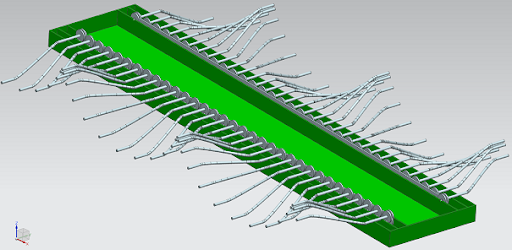
\includegraphics[width=0.33\linewidth]{strirus_0.png}}
        \hfill
        \subcaptionbox[List-of-Figures entry]{Вторая итерация, 12 ног, 2 DoF сегмент, непрерывная смена угла между лапками до 45 градусов\label{fig:strirus_1}}{%
            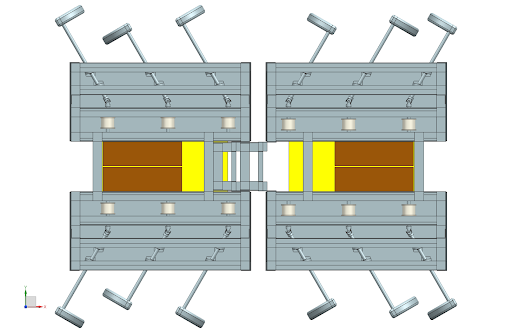
\includegraphics[width=0.33\linewidth]{strirus_1.png}}
        \hfill
        \subcaptionbox{Третья итерация, 12 ног, 2 DoF сегмент, дискретная смена угла между лапками до 45 градусов\label{fig:strirus_2}}{%
        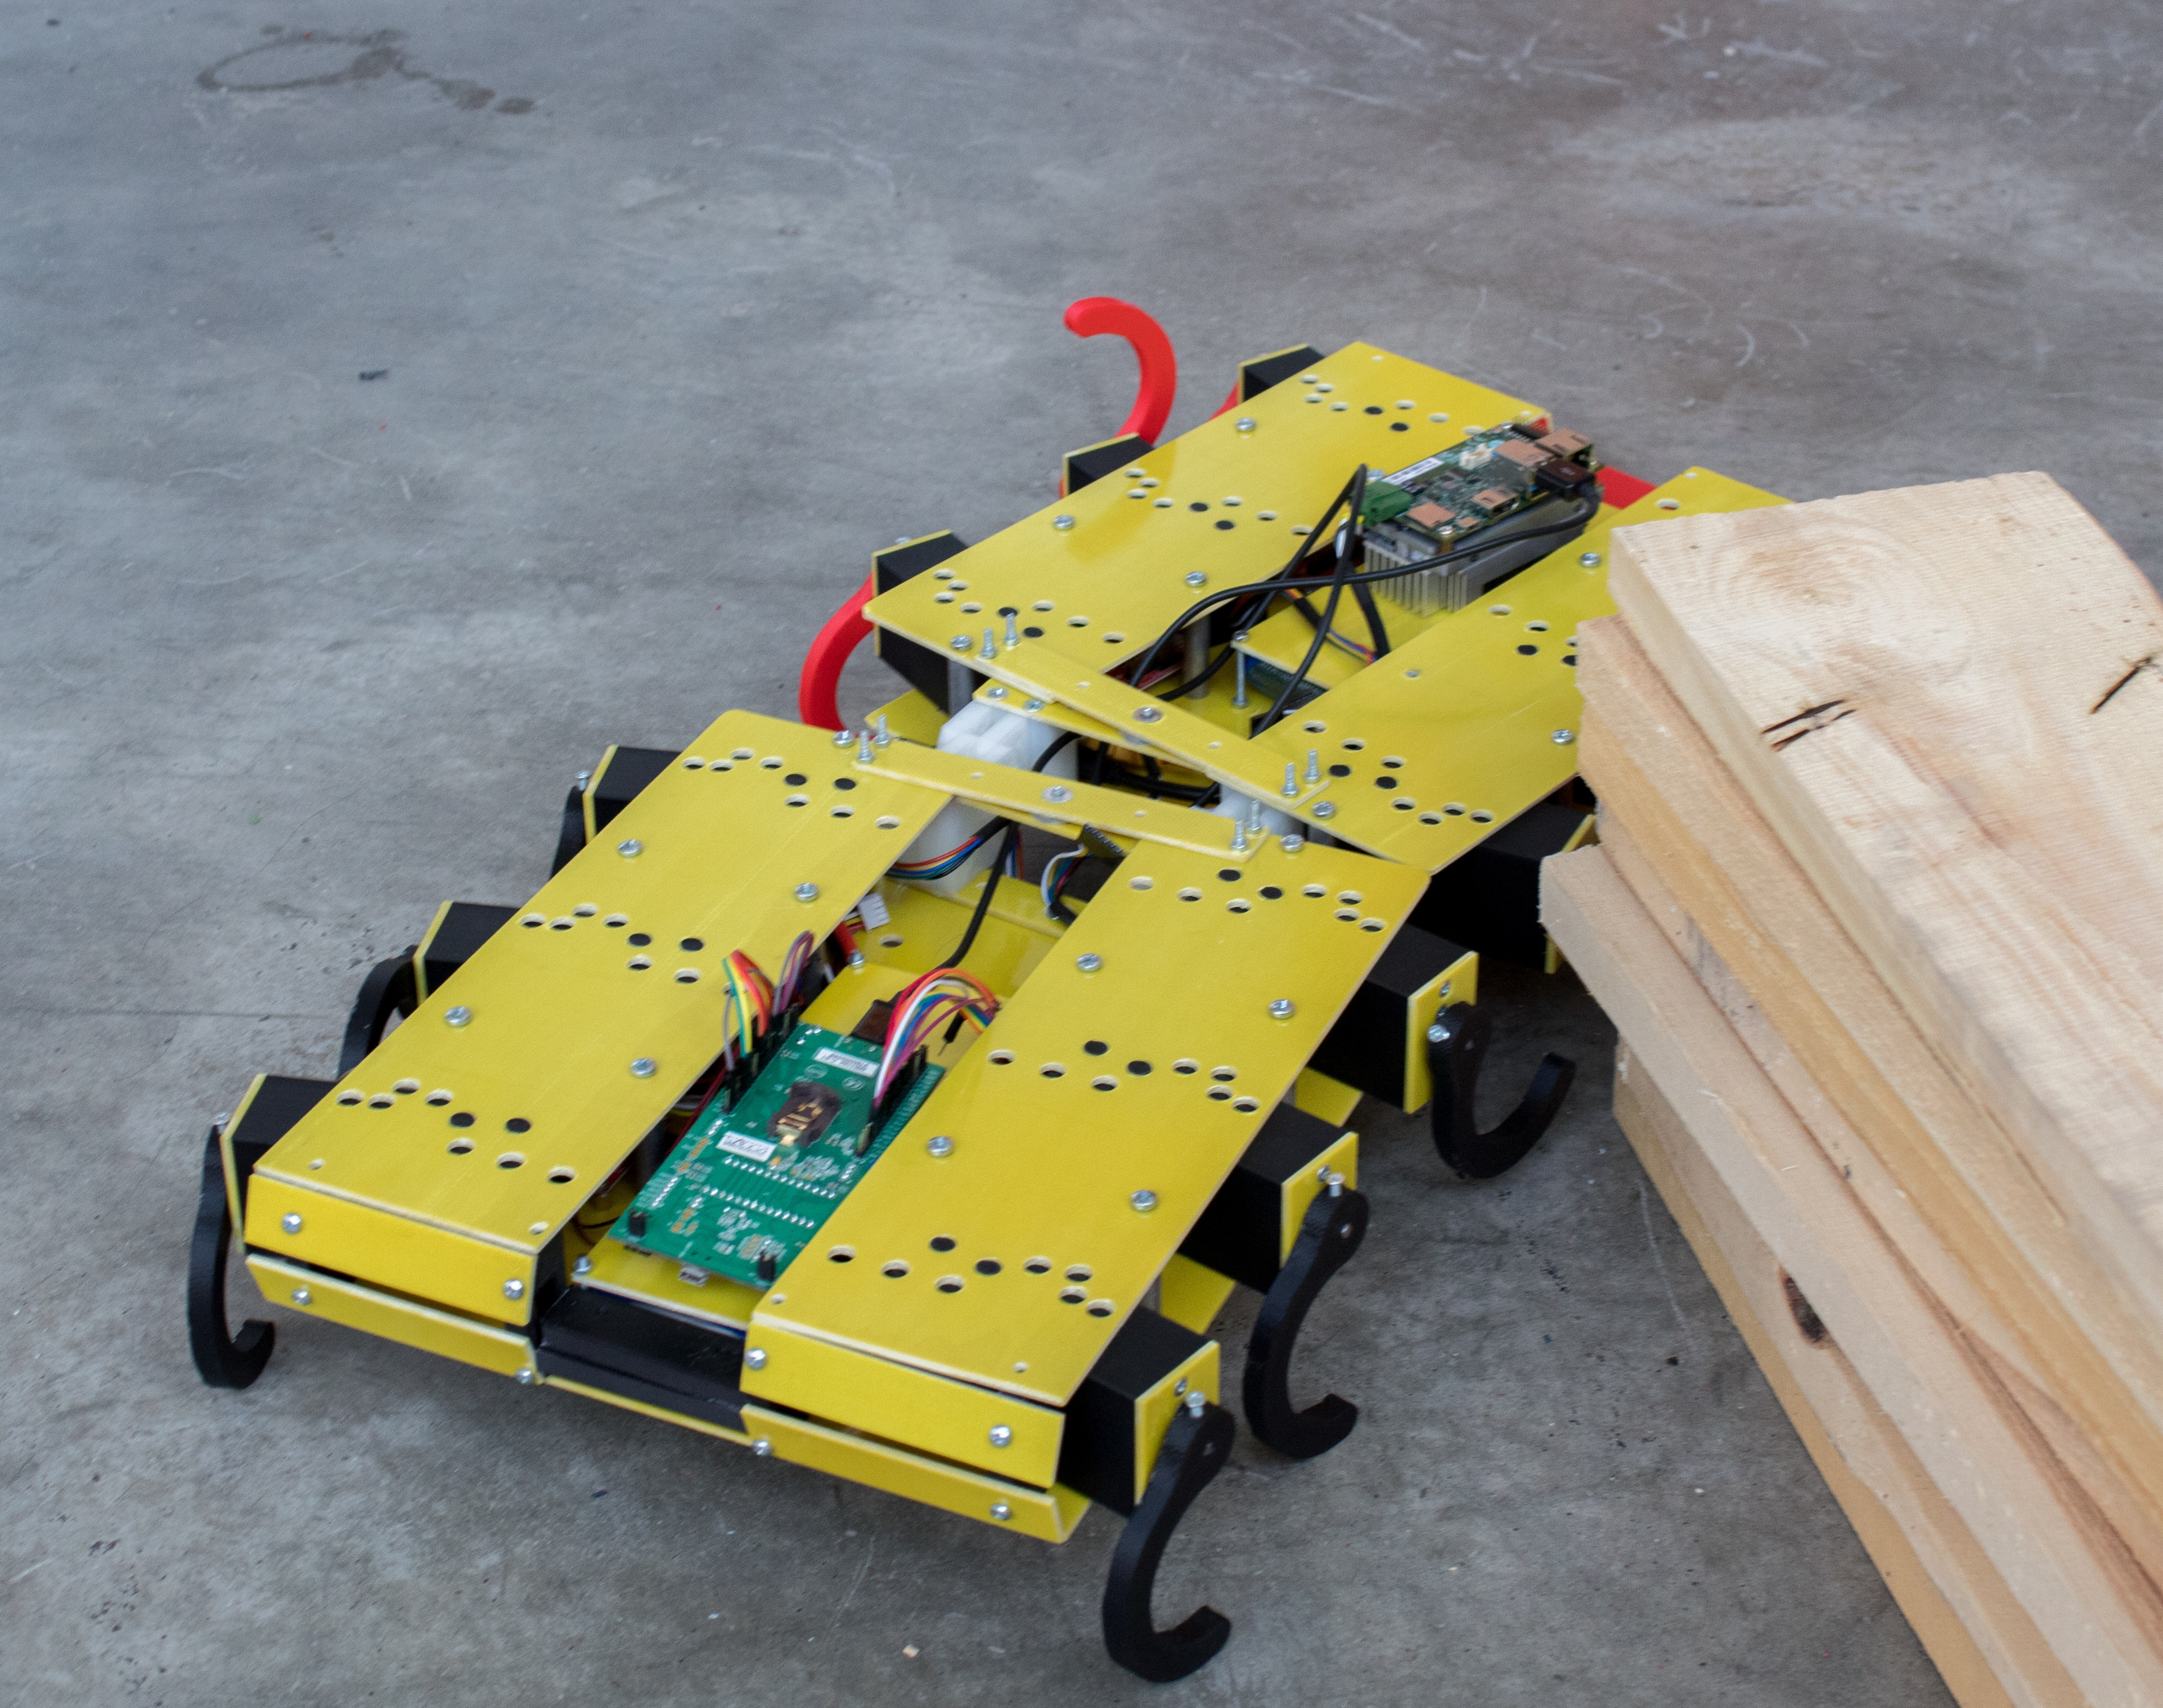
\includegraphics[width=0.33\linewidth]{strirus_2.jpg}}
        \hfill
        \subcaptionbox{Четвертая итерация, 6 ног, без сегмента, увеличенные ноги\label{fig:strirus_3}}{%
        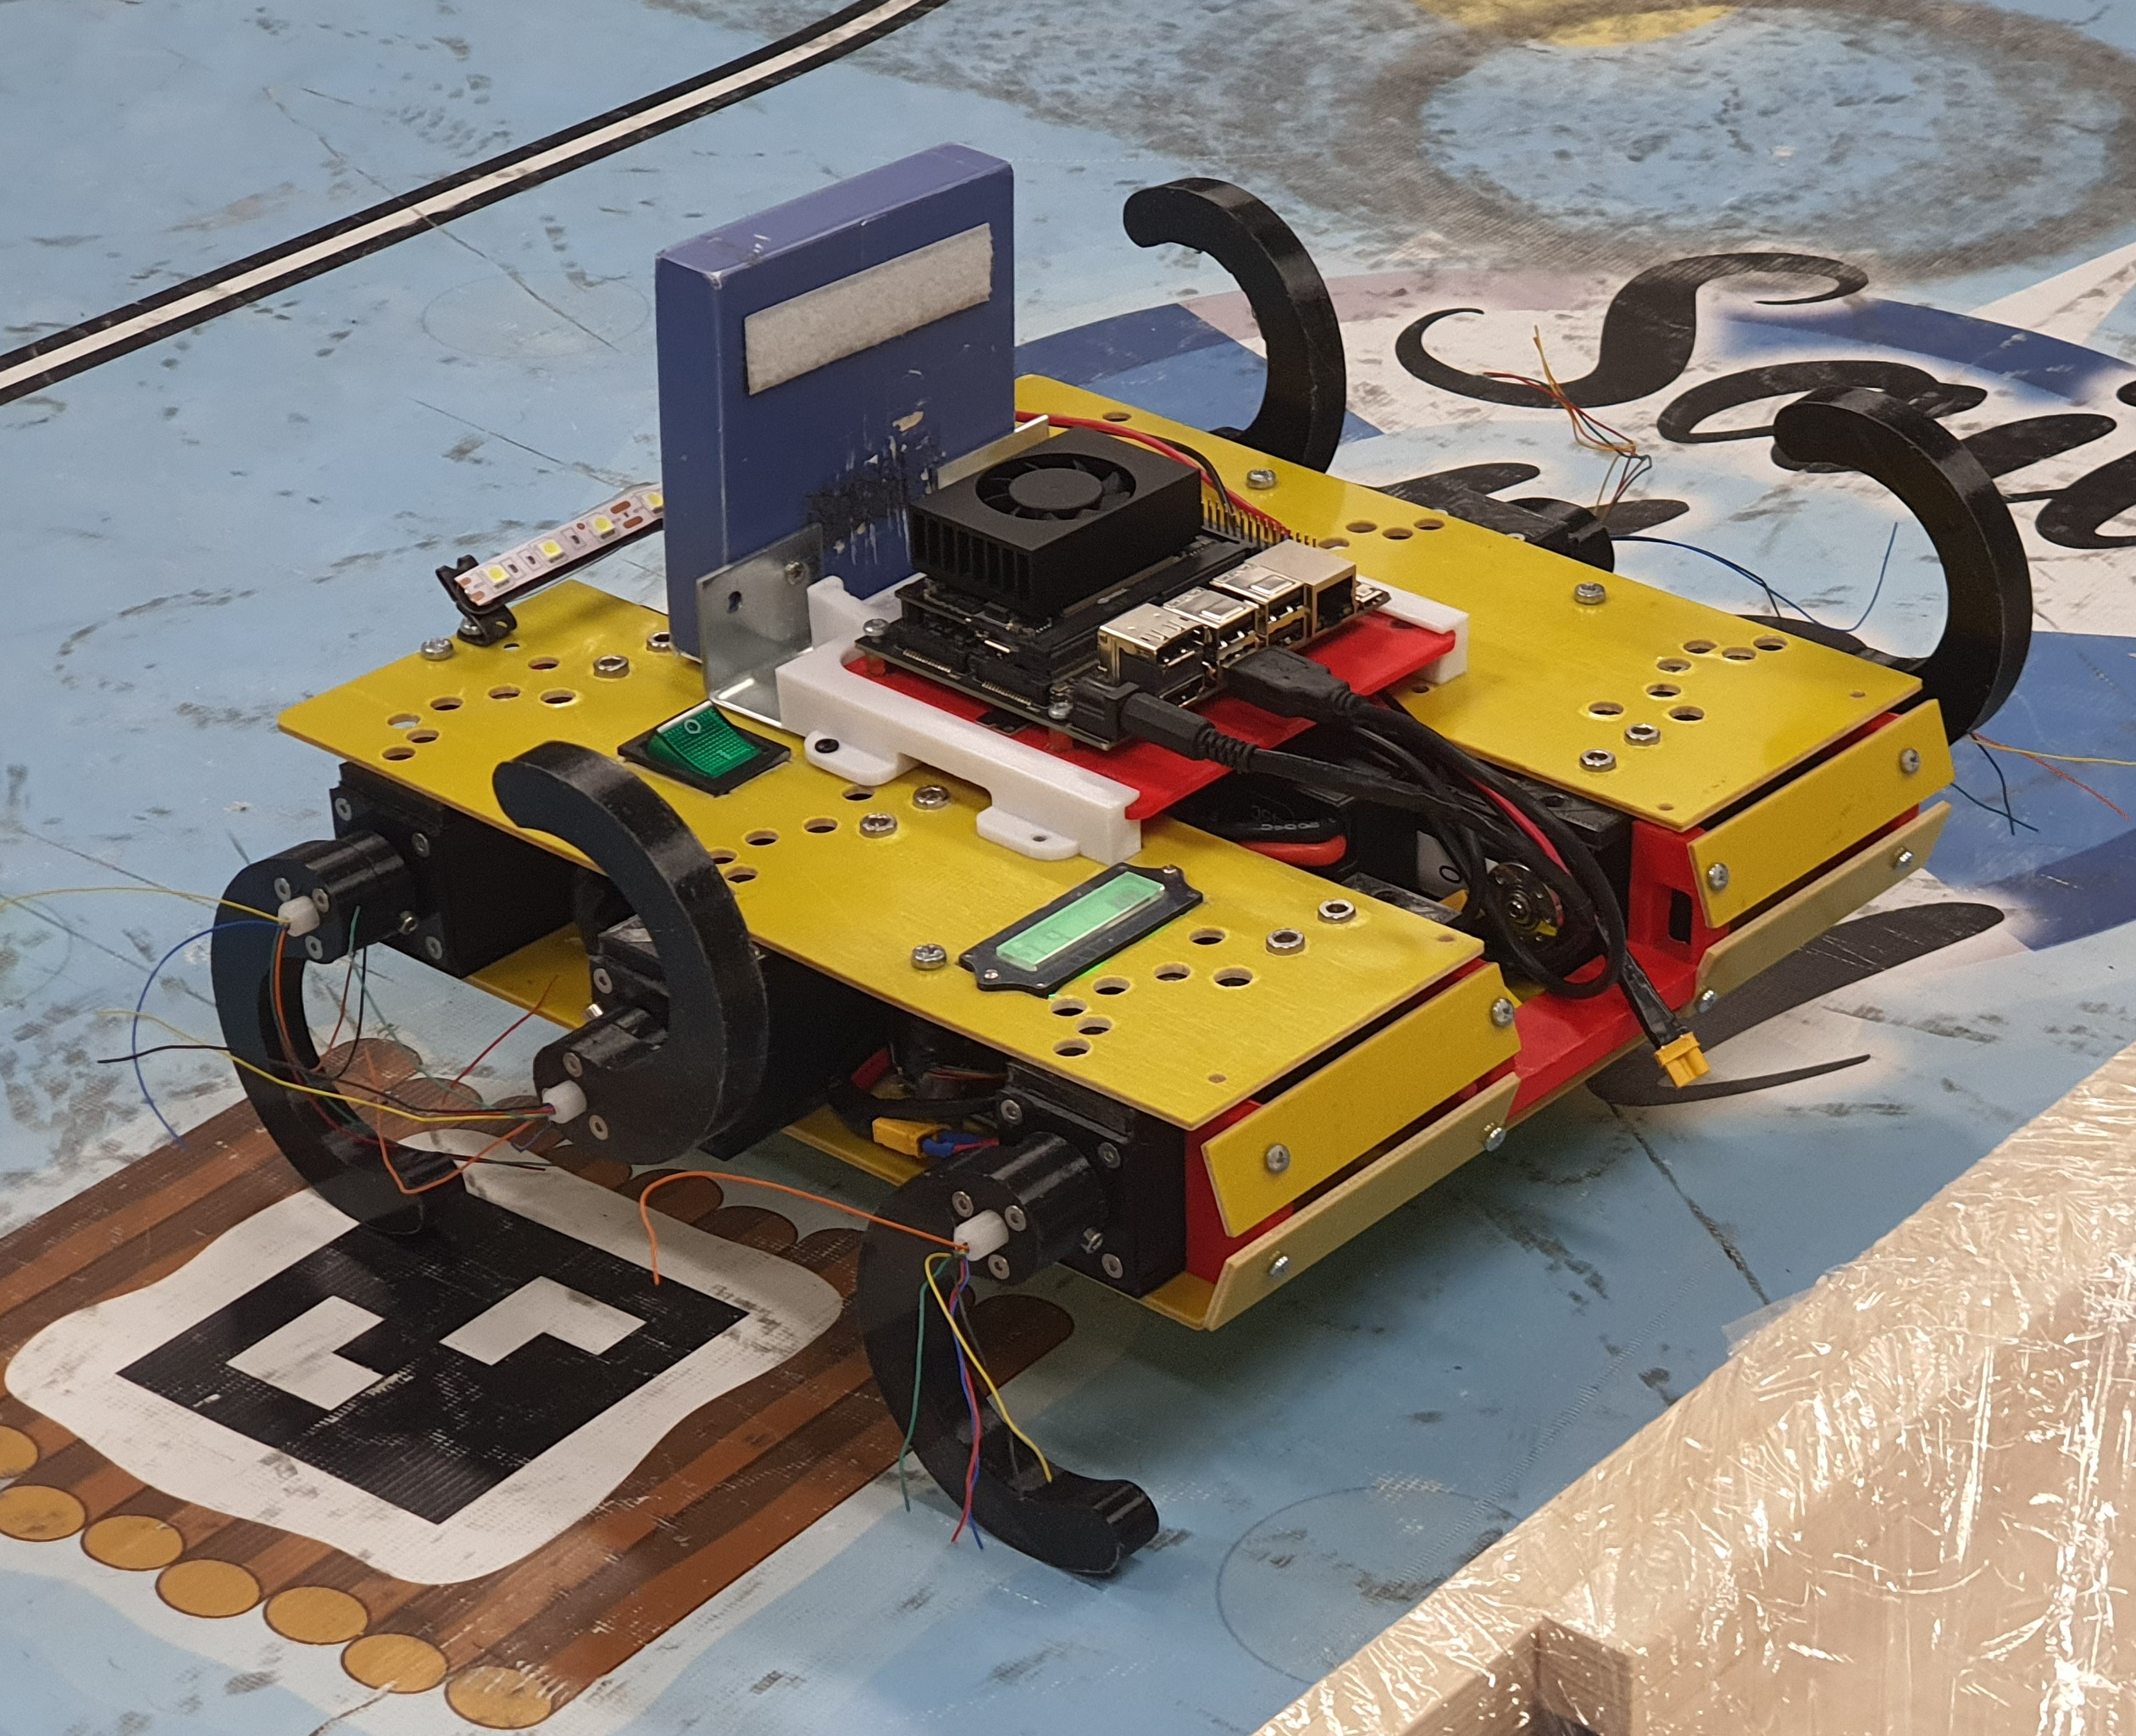
\includegraphics[width=0.45\linewidth]{strirus_3.JPG}}
        \hfill
        \subcaptionbox{Пятая итерация, 10 ног, 1 DoF сегмент, увеличенные ноги, дискретная смена угла между лапками на 15 градусов\label{fig:strirus_4}}{%
        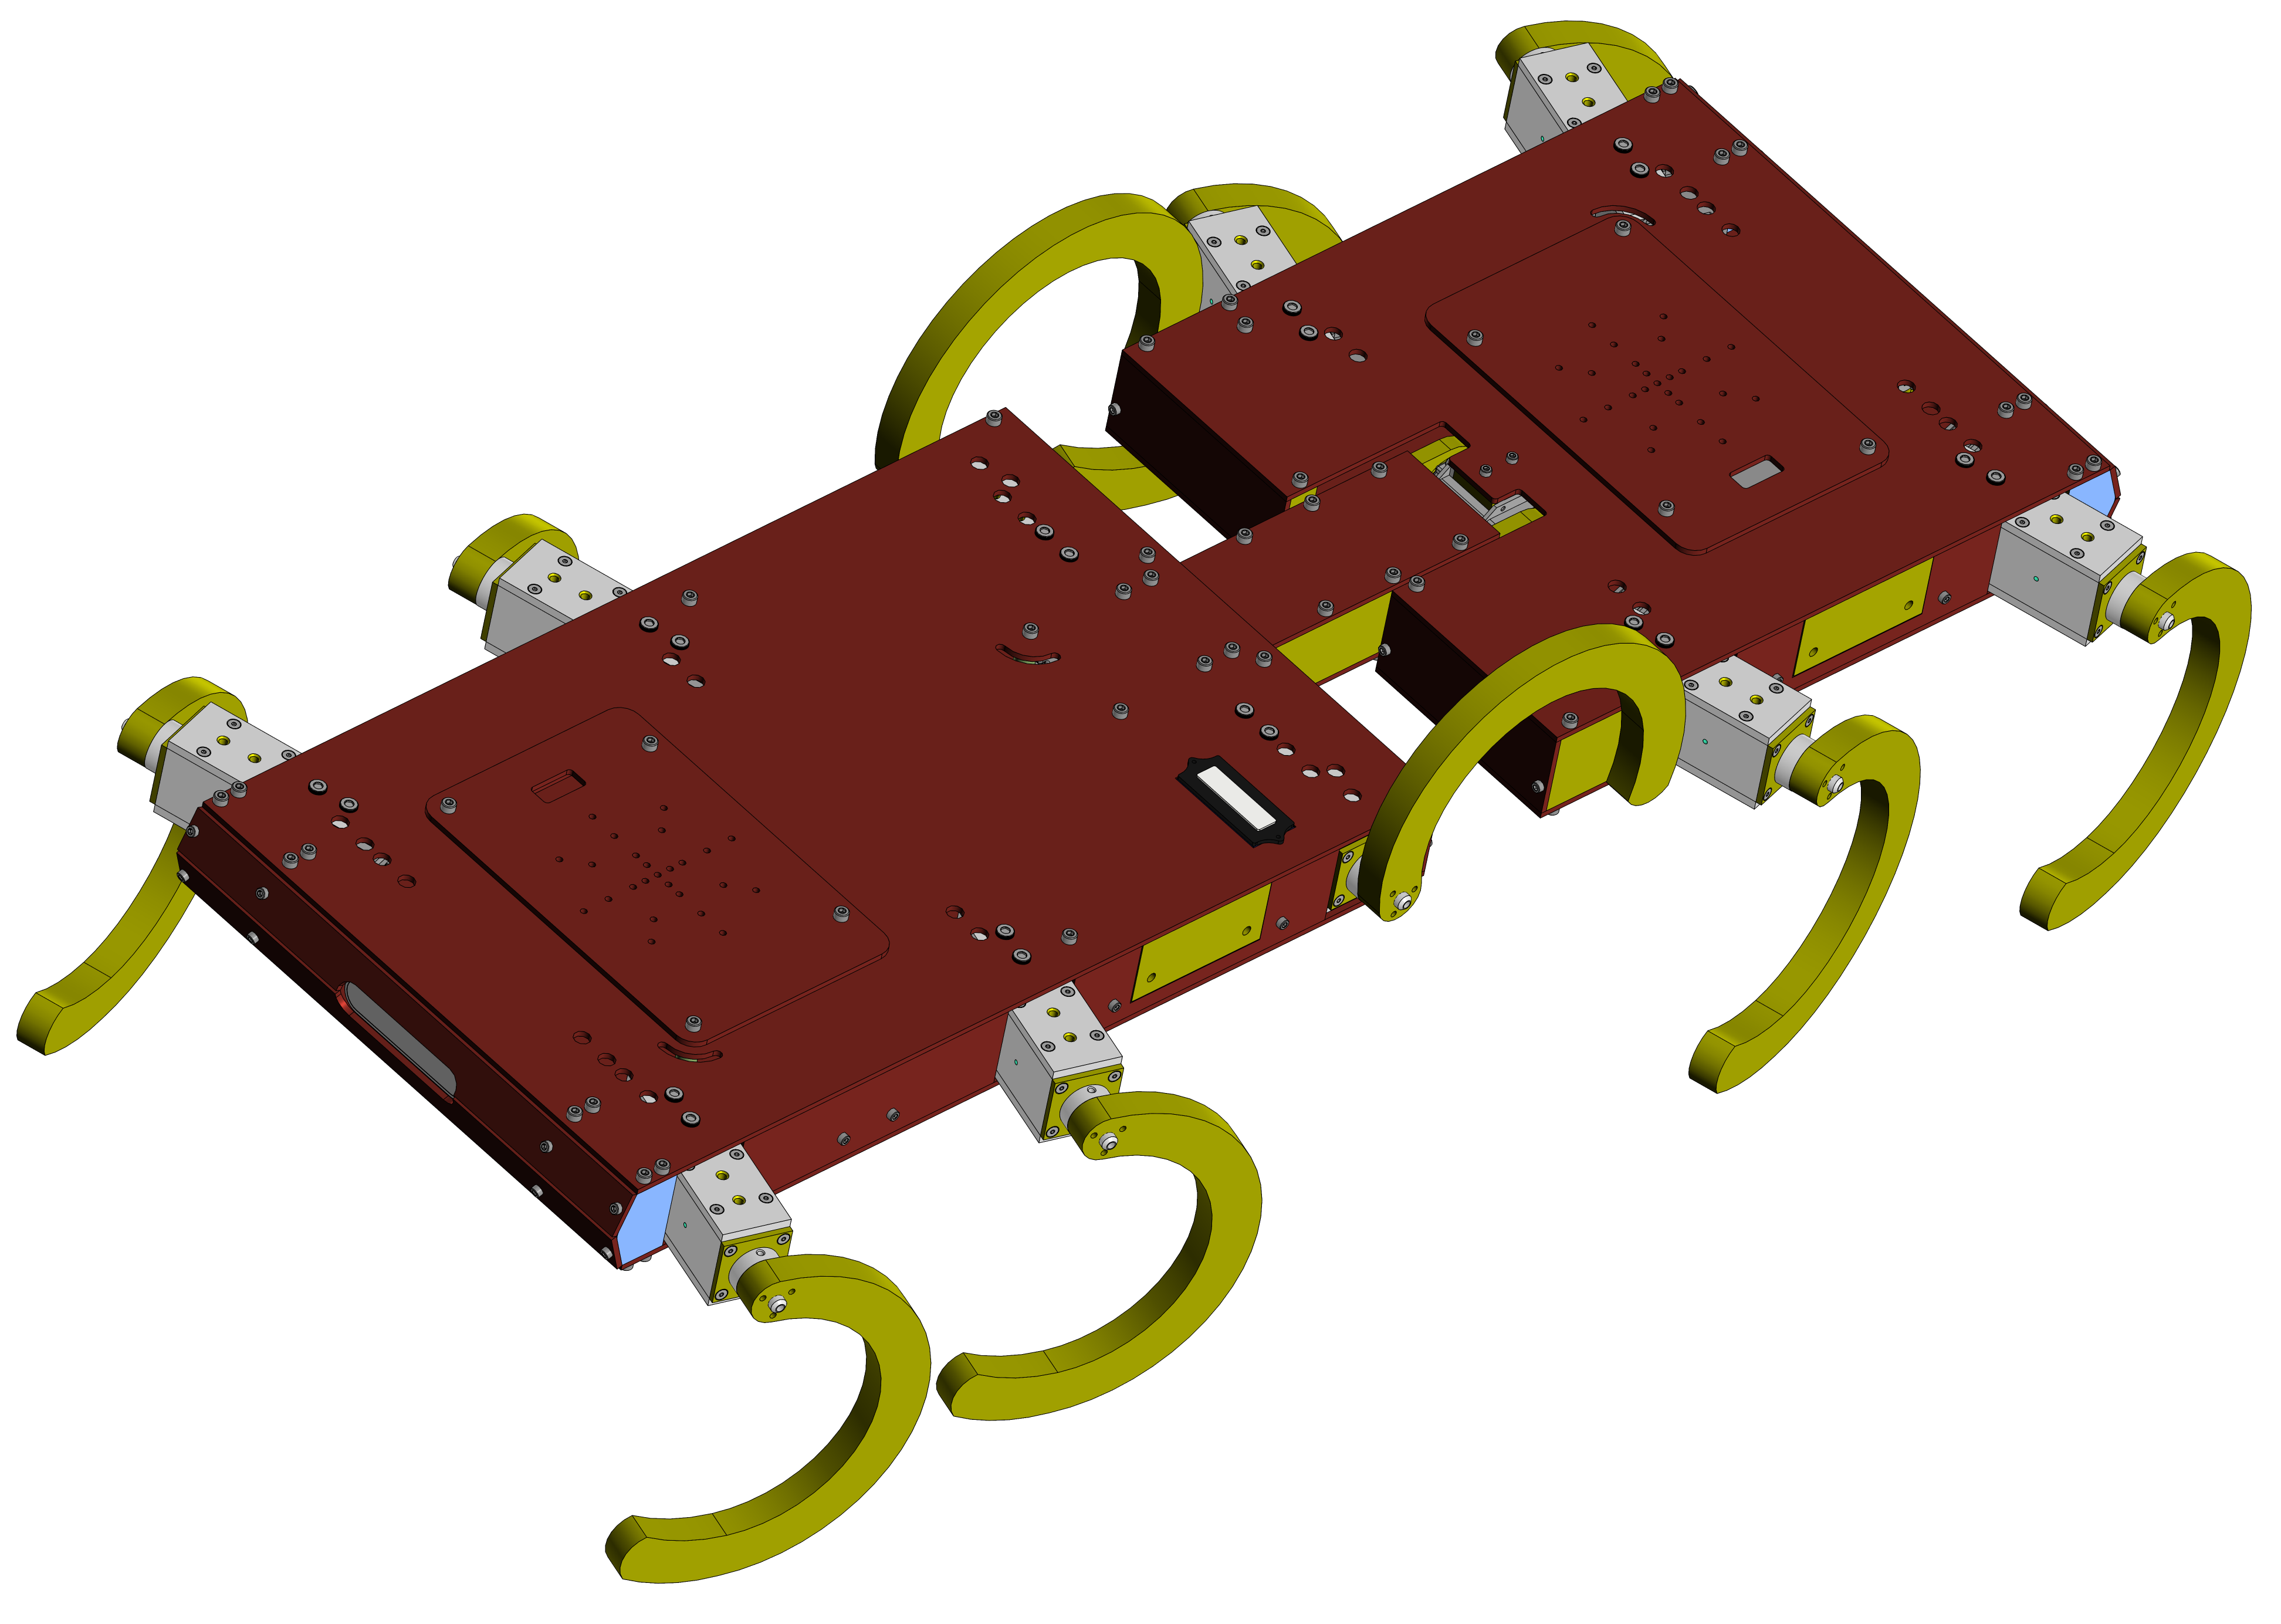
\includegraphics[width=0.45\linewidth]{strirus_4.png}}
    }
    % \legend{Подрисуночный текст, описывающий обозначения, например. Согласно
    %     ГОСТ 2.105, пункт 4.3.1, располагается перед наименованием рисунка.}
    \caption[Этот текст попадает в названия рисунков в списке рисунков]{Итерации робота СтриРуса}\label{fig:striruses}
  \end{figure}
  \vspace{-0.5cm}
